\section{Architecture}
\label{Architecture}
\subsection{Stakeholders}

\subsubsection{Customer}
Our goal with this course was to create a product that not only works the way the customer intended, but does so with satisfactory performance. It also needed a clear, logical and functional architecture to make it easy to maintain. 
Our code needed to be written following the clean coding standard and make use of interfaces and general polymorphism, so that their developers could further develop this solution with ease.

\subsubsection{Implementers}
We wanted an architecture that would be easy to implement and would make sense to the coders of our own team as well as to those of the customer.

\subsubsection{Course Staff}
The course staff wants a clear and well-documented architecture that is easy to understand and evaluate.


\subsection{Quality Attributes}
The customer was very specific when it came to what they wanted. % Were they, though? Rewrite/elaborate

\subsubsection{Modifiability}
While we were the create the solution for real estate ads specifically, the solution will be used for other ads as well. Therefore we need to make it modifiable so that other developers later on can further develop using our solution as a base.

\subsubsection{Performance}
We wanted the system to function with a satisfactory performance, even though the customer did not set any specific requirements for performance. For this reason, we decided to merely strive to achieve this goal by writing as efficient code as we could manage, making necessary changes to keep performance at a reasonable level. %Is this too vague?

\subsubsection{Availability}
The system should be available for the users when they need it. Therefore we needed to minimize the possible points of failure and the probability of these failing. % Too vague?

\subsubsection{Interoperability}
Our solution was only a part of the larger Webassistenten solution, and needed to inter-operate with already-existing order system. To achieve this goal, we used the same technology as requested by the customer, including Web API, MSSQL and so on.

\subsubsection{Readability}
The customer wants us to write readable code. The customer wants us to write interfaces and using polymorphism so other developers can develop it further by developing plug-ins for the system. Readability is therefore important for easier further development of this system.
%Whoever wrote this should probably rewrite it.

\subsection{Views}


\subsubsection{Process view}
There is no need for us to supply a process view, because we do not have access to their server. We are only supposed to write the code for their system, without taking into account how the processes inter-operate.
\subsubsection{Logical view}
\begin{figure}[H]
\centering
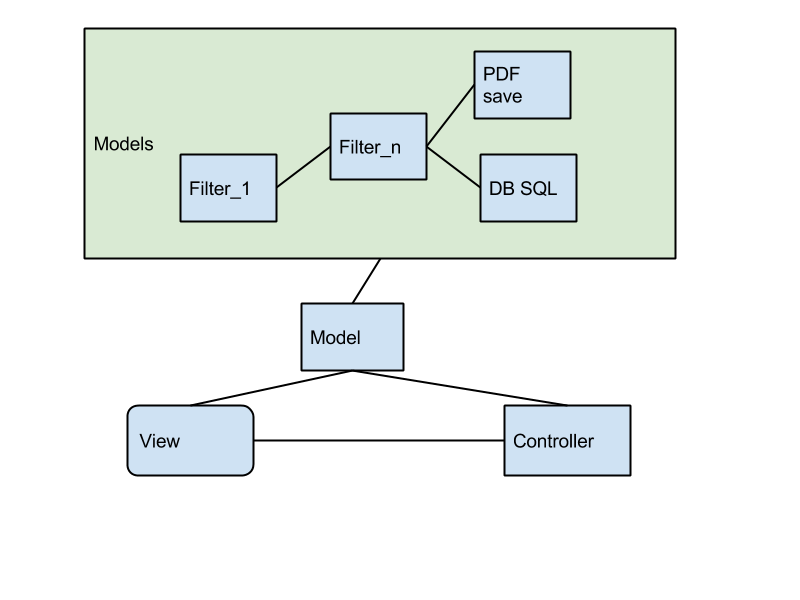
\includegraphics[width=0.8\textwidth]{images/architecture00.png}
\caption{Logical view}
\label{fig:logical_view}
\end{figure}
\newpage

\subsubsection{Scenario view}
\begin{figure}[H]
\centering
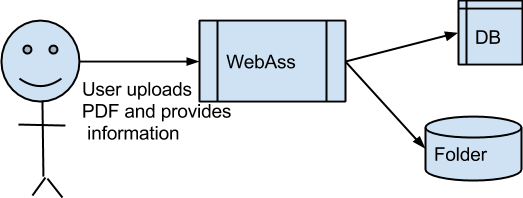
\includegraphics[width=0.8\textwidth]{images/architecture01.png}
\caption{Scenario view}
\label{fig:scenario_view}
\end{figure}




\subsubsection{Physical view}
\begin{figure}[H]
\centering
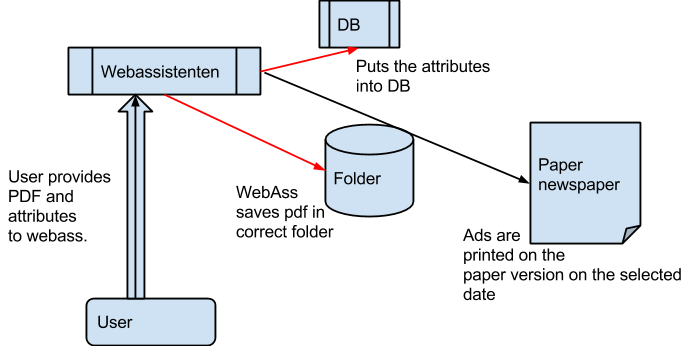
\includegraphics[width=0.8\textwidth]{images/architecture02.png}
\caption{Physical view, we implement the red arrows}
\label{fig:physical_view}
\end{figure}
\newpage
\subsection{Class diagram}
From these views, we made this class diagram.
\begin{figure}[H]
\centering
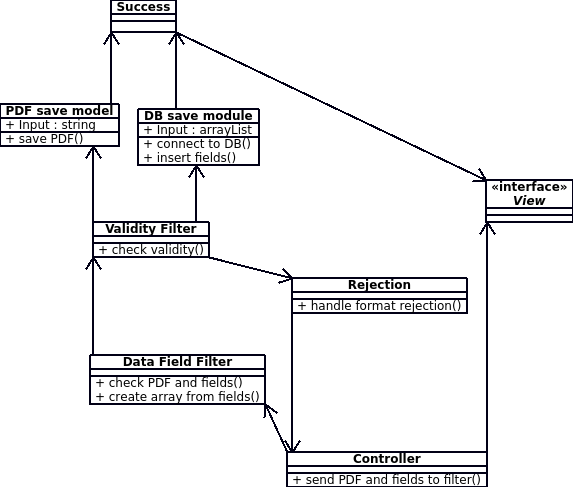
\includegraphics[width=0.8\textwidth]{diagrams/class_diagram.png}
\caption{Digital class diagram}
\label{fig:class_diagram}
\end{figure}
\subsection{Patterns}
MVC due to the technology and pipe \&  filter to filter the data and due to the modifiability requirement.
\subsection{Tactics}
\subsubsection{Modifiability}
\begin{itemize}
\item Increase semantic cohesion
\item Decrease coupling
\item Split modules
\end{itemize}

\subsubsection{Performance}
\begin{itemize}
\item Write optimal code
\end{itemize}

\subsubsection{Availability}
\begin{itemize}
\item Our code should not crash the customer's system, but it's their responsibility that the system is available.
\end{itemize}

\subsubsection{Interoperability}
\begin{itemize}
\item The technology and tools we're using should be sufficient to ensure interoperability.
\end{itemize}

\subsubsection{Readability}
\begin{itemize}
\item We will follow the clean coding principle and use camelCase coding. Refer to \ref{Templates and Standards section} Templates and Standards section on page \pageref{Templates and Standards section}
\end{itemize}

\subsection{Changes to the architecture}
When we started to implement the system we quickly found out that the we had architectural drift because the architecture we designed in the start didn't fit well into the web api framework. After we got an overview of the system we had change the architecture to a MVC pattern. 
\begin{figure}[H]
\centering
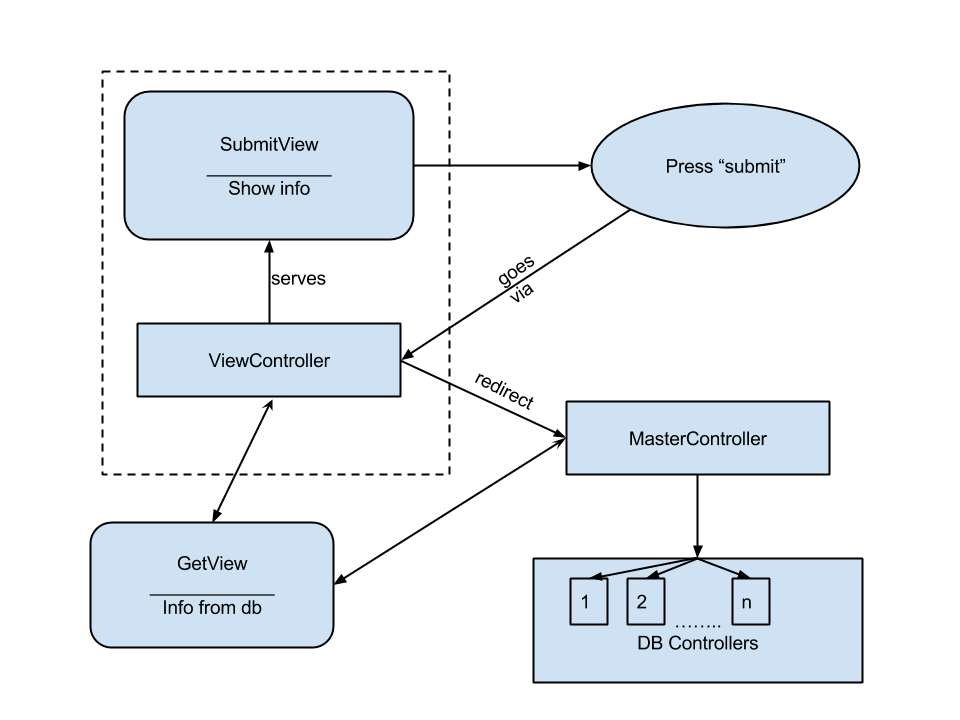
\includegraphics[width=0.8\textwidth]{images/architecture03_revised1.png}
\caption{New diagram showing the information flow}
\label{fig:info_flow}
\end{figure}
We tried to follow this MVC pattern when we implemented the system, however we quickly found out that the getView-Controller was not necessary.
\begin{center}
\begin{figure}[H]
\centering
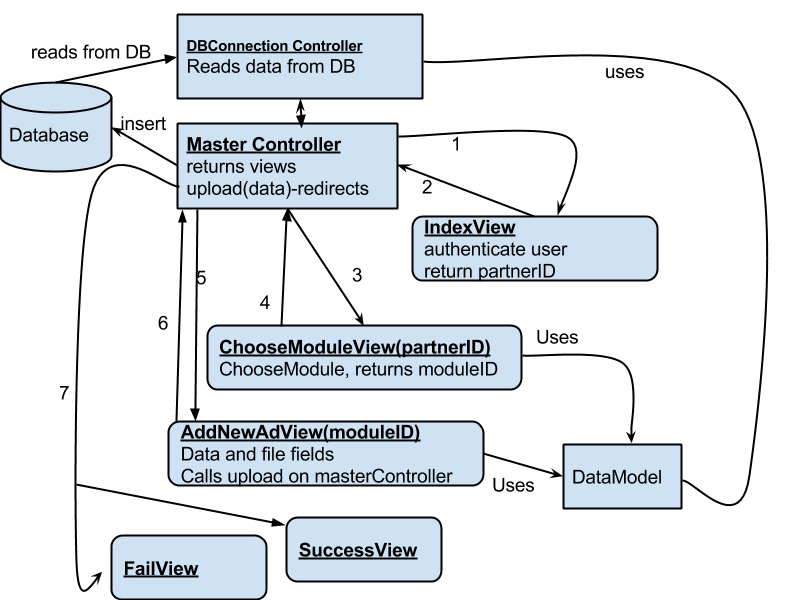
\includegraphics[width=0.8\textwidth]{images/architecture_final01.png}
\caption{The final architecture}
\caption*{6 calls the upload method with files and data\\
7 is the upload method redirecting either to a FailView or a SuccessView}
\label{fig:architecture}
\end{figure}
\end{center}
